\documentclass{article}


\usepackage{booktabs,array,multirow,amsmath,graphicx,xcolor}
\usepackage[a4paper, total={6in, 8in}]{geometry}
\usepackage{tikz}
\pagecolor{white}
\definecolor{fuchsia}{rgb}{1.0, 0.0, 1.0}
\definecolor{aqua}{rgb}{0.0, 1.0, 1.0}

\begin{document}

\begin{table}[h]
\begin{center}
\caption{Data of the scaling time for the approximation of $e$}
\begin{tabular}{lllll}
\toprule
Exercise   title      & e value            & \#thread & time [ms]          & \#pragma        \\
\toprule
ex\_e\_sequential.cpp & 2,71828182845899   & 1        & 0,000299032 & /               \\
ex\_e\_1.cpp          & 2,71828182845905   & 56       & 0,035678600 & Parallel        \\
ex\_e\_2.cpp          & 2,71828182845899   & 56       & 0,030270500 & For1            \\
ex\_e\_3.cpp          & 2,17661488659838   & 56       & 0,024728000 & For and For2    \\
ex\_e\_4.cpp          & 3,00000000000000   & 56       & 0,048437000 & Barrier and sum \\
ex\_e\_5.cpp          & 561,47991436235300 & 56       & 0,031016600 & Critical       \\
\bottomrule
\end{tabular}
\end{center}
\end{table}


\begin{figure}[h!]
  \caption{Scaling time for the approximation of $e$!}
  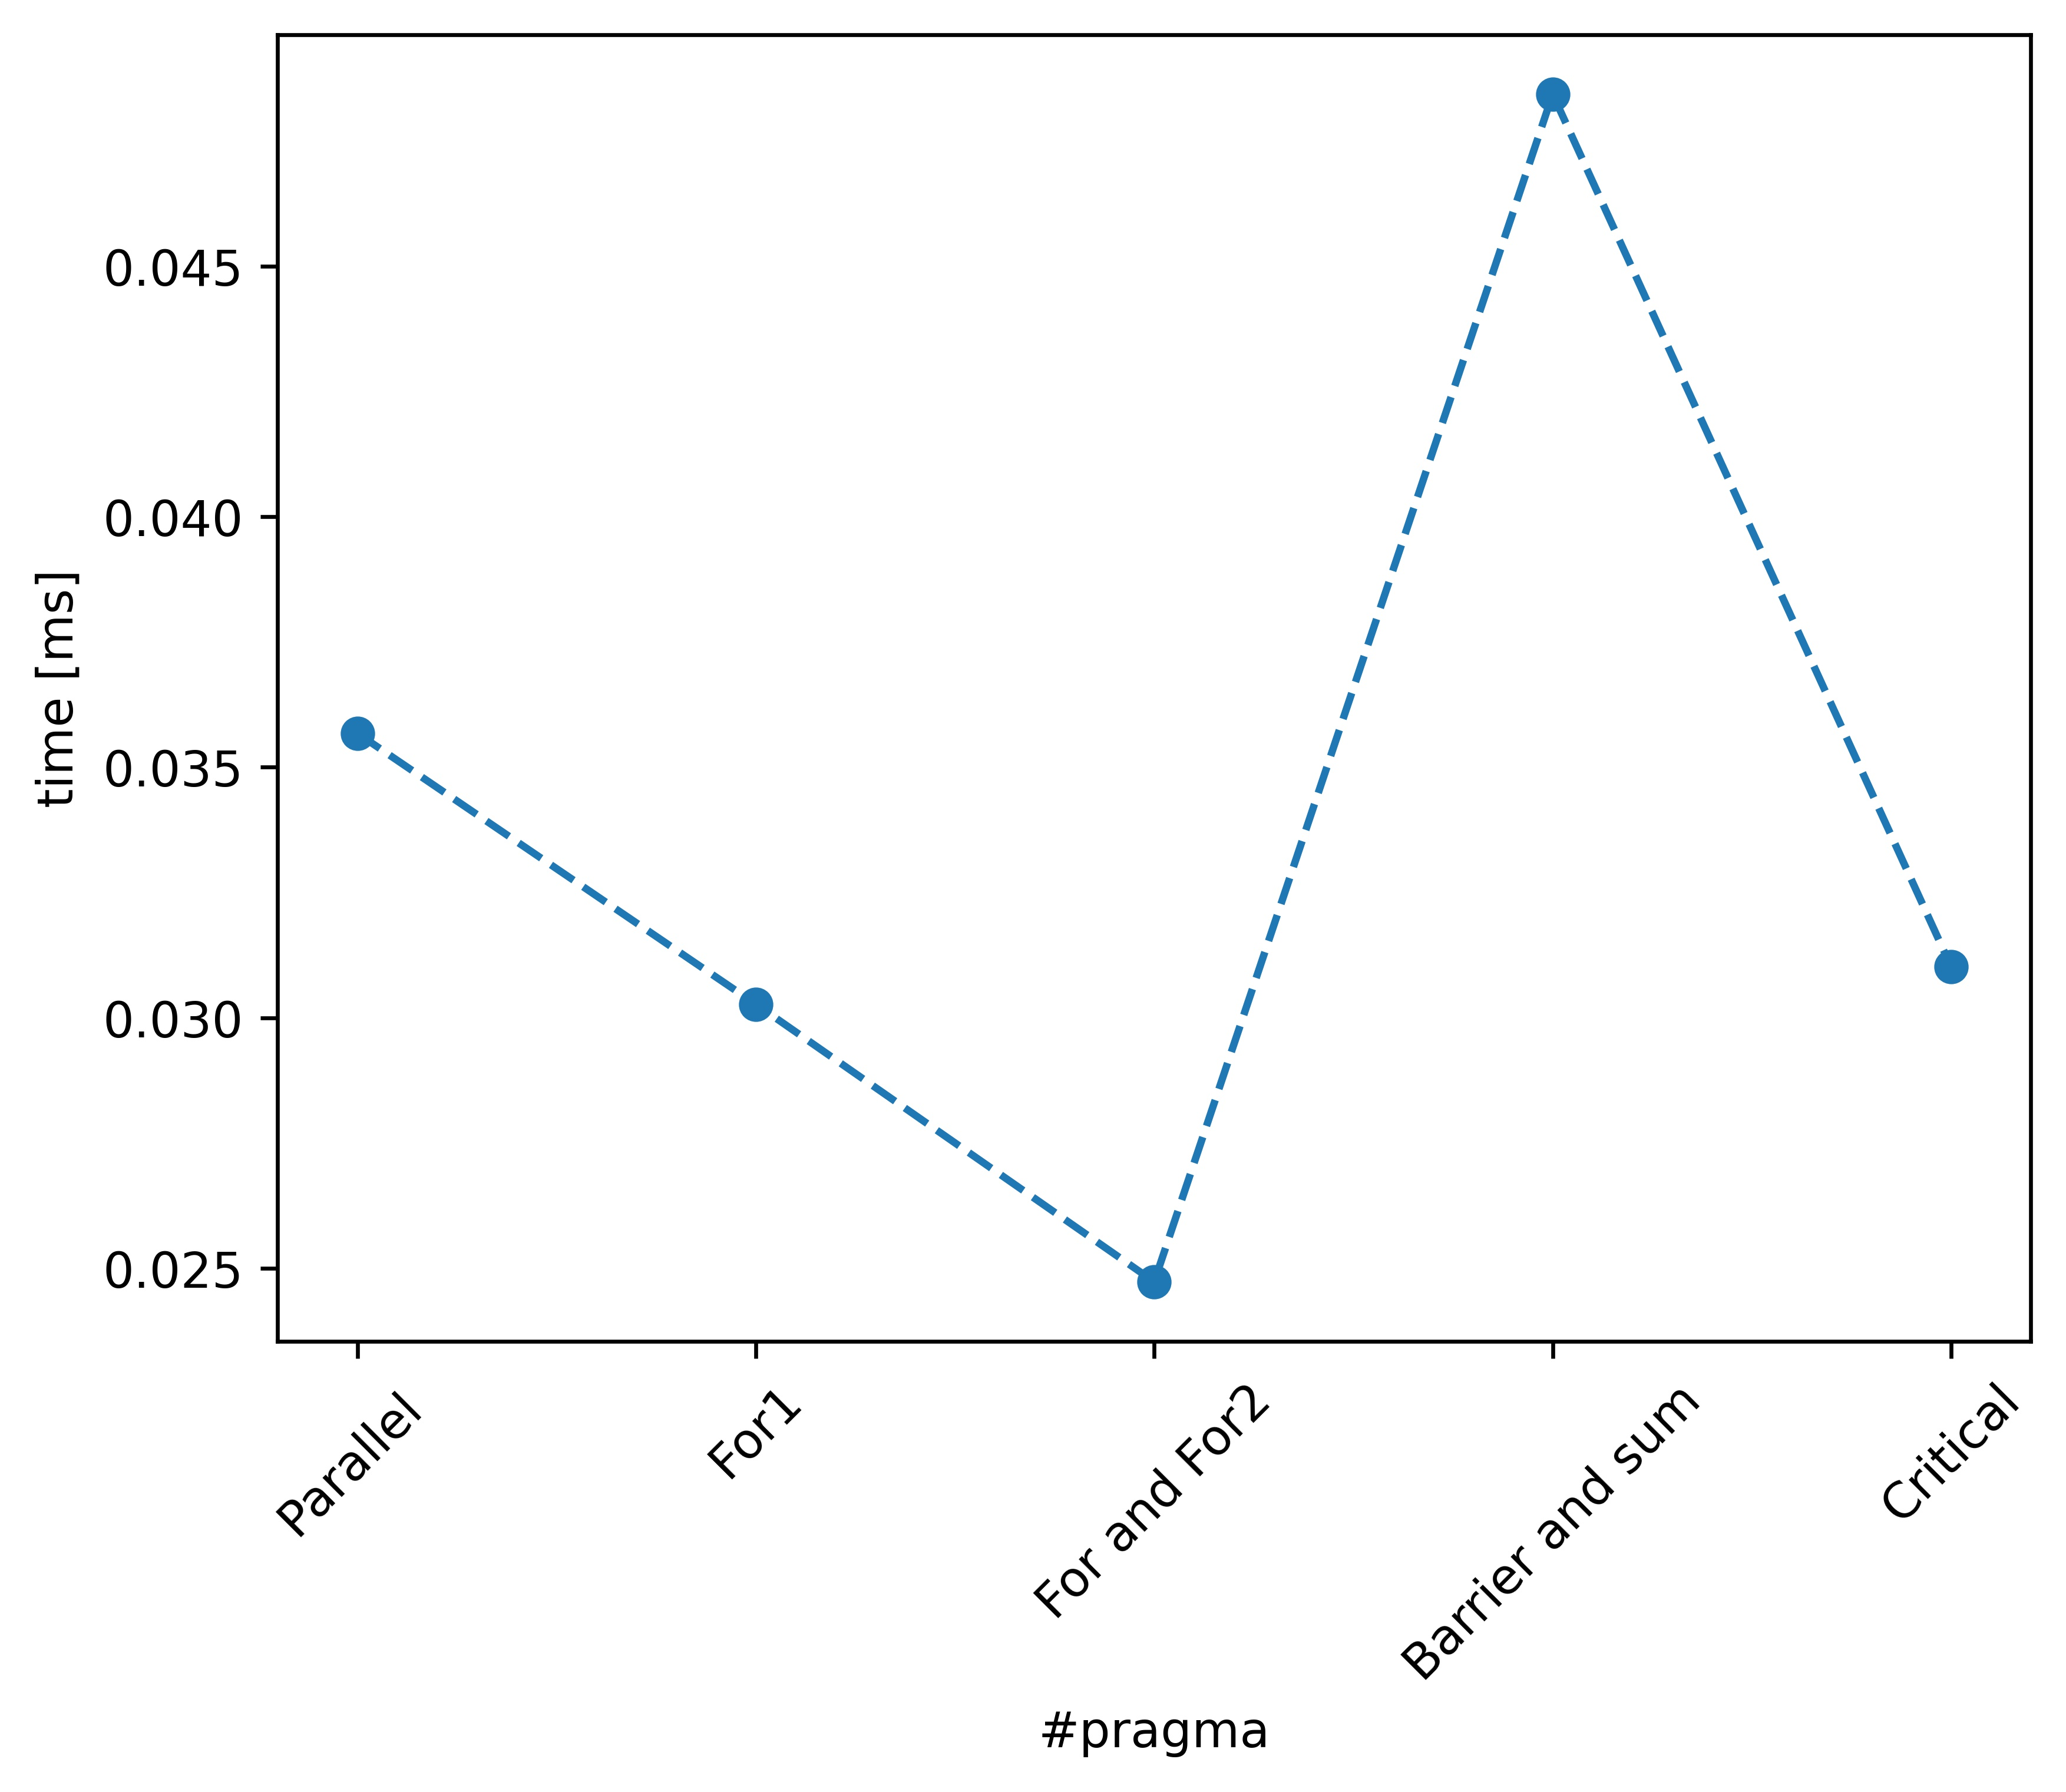
\includegraphics{e_time.jpg}
\end{figure}





\end{document} 